\documentclass[11pt]{article}
% =========================================================================
% SHARED STYLE FILE for 11_Master_Projects reports
% Visual style follows 0_Thesis_Submission/24m0553_AK_Gaurav_Mtech_Report.pdf:
% serif body font, blue hyperlinked TOC/links, ruled section headings,
% IITB-style title page, formal academic report structure.
% =========================================================================

\usepackage[a4paper,margin=1in]{geometry}
\usepackage{xcolor}
\usepackage{graphicx}
\graphicspath{{../images/}}
\usepackage{amsmath,amssymb}
\usepackage{booktabs}
\usepackage{caption}
\usepackage{float}
\usepackage[hidelinks]{hyperref}
\usepackage{titlesec}
\usepackage{enumitem}
\usepackage{setspace}
\usepackage[T1]{fontenc}
\usepackage{lmodern}
\usepackage{microtype}

% Every \includegraphics call is automatically framed with a thin black
% border (matches the printed look of figures/photos/charts in the source
% reports). \oldincludegraphics is kept available for institutional
% logos/seals on title pages, which should remain unframed.
\let\oldincludegraphics\includegraphics
\setlength{\fboxsep}{1pt}
\setlength{\fboxrule}{0.6pt}
\renewcommand{\includegraphics}[2][]{\fbox{\oldincludegraphics[#1]{#2}}}

\definecolor{thesisblue}{RGB}{0,0,205}
\hypersetup{
  colorlinks=true,
  linkcolor=thesisblue,
  urlcolor=thesisblue,
  citecolor=thesisblue,
  filecolor=thesisblue
}

\onehalfspacing
\setlength{\parskip}{6pt}
\setlength{\parindent}{0pt}

\titleformat{\section}
  {\normalfont\Large\bfseries}{\thesection}{1em}{}
\titleformat{\subsection}
  {\normalfont\large\bfseries}{\thesubsection}{1em}{}
\titleformat{\subsubsection}
  {\normalfont\normalsize\bfseries}{\thesubsubsection}{1em}{}

\newcommand{\reportTitlePage}[7]{%
  % #1 = Report title
  % #2 = Course code & name (e.g. "CE 605: Applied Statistics")
  % #3 = Subtitle/topic line (e.g. "Project Report 2: Network Analysis")
  % #4 = Author block (can be multi-line with \\ for group projects)
  % #5 = Supervisor name(s)
  % #6 = Programme line (e.g. "M.Tech in Transportation Systems Engineering")
  % #7 = Month/Year
  \begin{titlepage}
    \centering
    \vspace*{0.5cm}
    {\large\bfseries #2}\par
    \vspace{0.3cm}
    {\Large\bfseries #3}\par
    \vspace{1.2cm}
    {\Huge\bfseries #1}\par
    \vspace{1.5cm}
    \oldincludegraphics[width=3.2cm]{../../assets/iitb_logo.png}\par
    \vspace{1.2cm}
    Submitted by:\par
    \vspace{0.2cm}
    {\bfseries #4}\par
    \vspace{0.8cm}
    Under the Supervision of\par
    \vspace{0.2cm}
    {\bfseries #5}\par
    \vspace{1.2cm}
    #6\par
    Department of Civil Engineering\par
    \textbf{Indian Institute of Technology Bombay}\par
    Mumbai -- 400076, India\par
    \vspace{0.3cm}
    #7\par
  \end{titlepage}
}

\newcommand{\reportAbstract}[1]{%
  \section*{Abstract}
  #1
  \vspace{0.5cm}
}

\usepackage{longtable}

\title{Sensitivity Analysis and Operational Improvement Strategies for the H10 T-Junction, IIT Bombay Campus}
\author{Abhijeet Kumar Gaurav et al.}
\date{}

\begin{document}

\begin{titlepage}
\centering
\vspace*{0.2cm}
{\Large\bfseries\underline{CE 774: Traffic Management and Design}}\par
\vspace{0.3cm}
{\large Coursework Project Report}\par
\vspace{0.15cm}
{\large\bfseries\underline{Topic: Sensitivity Analysis at the H-10 Junction, IIT Bombay}}\par
\vspace{0.8cm}
submitted by:\par
\vspace{0.15cm}
{\small
Abhijeet Kumar Gaurav, 24M0553\\
Lekshmi Murlidharan, 24M0544\\
Deep Medatwal, 210040044\\
Deven Ratnaparkhi, 210040045\\
Harendra Pratap Singh Baghel, 210040054\\
Kartik Khandelwal, 210040072\\
Mariyam Saqib, 210040090\\
Mohak Gupta, 210040097\par
}
\vspace{0.6cm}
Supervisor:\par
\vspace{0.1cm}
{\bfseries Professor Archak Mittal}\par
\vspace{0.5cm}
TA Guides:\par
\vspace{0.1cm}
{\small Aiswaryabsree, Dhaval Barot, Manju Putra Pratyush, Shyam Manchhani, Vaishnavi Shinde}\par
\vspace{0.7cm}
\oldincludegraphics[width=2.3cm]{../../assets/iitb_logo.png}\par
\vspace{0.5cm}
Department of Civil Engineering\par
\textbf{Indian Institute of Technology Bombay}\par
Mumbai, 400076, India\par
\vspace{0.2cm}
Spring 2025\par
\end{titlepage}

\pagenumbering{roman}

\reportAbstract{
Rapid infrastructural development within the IIT Bombay (IITB) campus, including new hostel
construction and drainage works, has increased vehicular activity and reduced effective road space
near the H10 intersection, causing operational inefficiencies. This study evaluates the current and
projected traffic performance of the unsignalised H10 T-junction using microsimulation modelling in
PTV VISSIM. A baseline model, calibrated to reflect existing traffic conditions, was used to simulate
future scenarios with 2\%, 5\%, and 7\% traffic increments. Sensitivity analysis assessed the
intersection's performance in terms of travel time, vehicle delay, queue length, fuel consumption, and
Level of Service (LOS). The base scenario indicated severe congestion, with movements from the Energy
Building side operating at LOS~F and experiencing high delays and queue lengths. Two improvement
strategies were evaluated: widening of approach lanes and the introduction of dedicated cycle tracks.
Lane widening reduced average travel times by 34 to 50\%, delays by up to 75\%, and fuel consumption by
70 to 80\%. Dedicated cycle lanes dramatically reduced delays and queues for multiple movements,
yielding fuel savings of nearly 99\% for some approaches. Signalisation was ruled out per IRC:93
guidelines, as traffic volumes and operational characteristics did not warrant a traffic signal. The
study concludes that targeted non-signalised improvements, particularly geometric modification and
modal segregation, can significantly enhance the operational efficiency and safety of the H10
intersection, offering a practical framework for future campus mobility planning.

\vspace{0.3cm}
\noindent\textbf{Keywords:} PTV VISSIM Microsimulation; Unsignalised Intersection; Sensitivity Analysis;
Level of Service; Lane Widening; Dedicated Cycle Tracks; Campus Traffic Planning
}

\newpage
\tableofcontents
\newpage
\pagenumbering{arabic}

\section{Introduction}

\subsection{Background}
Urban campuses such as IIT Bombay (IITB) experience evolving and dynamic traffic patterns due to
continuous infrastructural expansion and growing student and staff populations. Ongoing construction
activities, including new hostel blocks and drainage works near Hostel~10 (H10), are expected to
substantially increase vehicular and pedestrian movement in and around the primary corridors of the
campus.

Intersections are critical points within any traffic network, where multiple streams of traffic meet
and interact. Unsignalised intersections depend heavily on driver behaviour, sight distance, and
negotiated priority. Without proper assessment and management, such intersections are vulnerable to
congestion, operational delays, and safety risks.

One such important location on the IIT Bombay campus is the H10 T-junction, where routes from Hostel~10,
the main academic area, and residential sectors converge. Given the anticipated rise in traffic demand,
there is a need to systematically evaluate the operational performance of this intersection.

\subsection{Motivation}
The H10 intersection is a vital connection point linking hostels, academic buildings, and
administrative areas. Several factors currently challenge its operational efficiency:
\begin{itemize}
  \item \textbf{Proximity to key landmarks:} the intersection lies adjacent to KV School and the
  Infinity Corridor entrance, both contributing high pedestrian and vehicular flows.
  \item \textbf{Rising pedestrian movements:} increased entrances to Hostel~10 have raised footfall,
  including young students, emphasising the need for pedestrian safety.
  \item \textbf{Traffic and visibility challenges:}
  \begin{itemize}
    \item Construction activities have resulted in a higher influx of heavy commercial vehicles (HCVs)
    and auto-rickshaws.
    \item Roadway space has been reduced due to ongoing drainage works, affecting the effective
    carriageway width.
    \item The existing Hostel~10 building obstructs sight distances at the junction, complicating
    manoeuvring for both vehicles and pedestrians.
    \item Planned new hostels (H19, H21, etc.) are likely to further escalate traffic volumes in the
    near future.
  \end{itemize}
\end{itemize}
Given these challenges, it becomes imperative to evaluate existing traffic conditions at the H10
intersection and explore potential improvement strategies. Using microsimulation tools like PTV VISSIM,
various operational strategies, such as road layout changes, pedestrian crossing improvements, and
possible geometric redesigns, can be tested in a virtual environment before implementation. This
approach ensures evidence-based planning and enhances both vehicular and pedestrian safety within the
campus.

\subsection{Problem Statement}
The ongoing infrastructural developments within the IIT Bombay campus have significantly altered
existing traffic dynamics around the H10 intersection. The main challenges observed are:
\begin{itemize}
  \item Increased vehicular movement, particularly of autos and heavy commercial vehicles (HCVs),
  related to construction activities.
  \item Reduction in effective road width due to drainage construction, leading to restricted vehicular
  movement space.
  \item Emergence of localised congestion during peak hours, caused by both the increased volume and
  reduced carriageway width.
  \item Limited sight distance near the H10 junction, making vehicle turning manoeuvres riskier and
  slowing down overall traffic movement.
\end{itemize}
Combined, these factors contribute to operational inefficiencies at the unsignalised H10 intersection.
Thus, a detailed operational analysis is necessary to assess current traffic performance under
constrained roadway conditions, simulate future scenarios considering ongoing and planned developments,
and identify and recommend feasible improvements to enhance intersection performance and safety.

\subsection{Objectives}
The primary objectives of this study are:
\begin{enumerate}
  \item To develop a calibrated microsimulation model of the H10 unsignalised intersection using PTV
  VISSIM.
  \item To evaluate the current operational performance in terms of travel time, delay, and queue
  length.
  \item To simulate future traffic scenarios incorporating projected traffic growth (assumed at 3\%
  annually for five years).
  \item To perform sensitivity analysis to assess intersection performance under increased traffic
  conditions.
  \item To recommend feasible short-term and long-term measures for enhancing intersection operations
  and safety.
\end{enumerate}

\subsection{Scope of the Study}
\begin{itemize}
  \item The study area is limited to the H10 T-junction, considering traffic inflows and outflows from
  the Main Gate, H17, and Energy Building directions.
  \item The current infrastructure setup, without any significant geometric changes, is considered in
  the base model.
  \item Pedestrian inflow is discussed qualitatively based on field observations; dedicated pedestrian
  simulation is not performed in this phase.
  \item Microsimulation modelling focuses on the current and projected traffic scenarios without
  assuming any additional traffic control installations (e.g.\ signals) in the base case.
\end{itemize}

\subsection{Significance of the Study}
Analysing the operational performance of the H10 intersection is crucial for maintaining efficient
campus mobility, particularly in the context of rapid campus expansion. This study provides:
\begin{itemize}
  \item A data-driven foundation for making informed campus traffic management decisions.
  \item Insight into the impact of construction-related disruption on traffic operations.
  \item A practical case study demonstrating the application of microsimulation tools like PTV VISSIM
  for small-scale intersection analysis.
  \item Recommendations that can be immediately applicable to IIT Bombay and extendable to other
  institutional or urban campuses facing similar congestion challenges.
\end{itemize}
The findings of this study aim to enhance safety, optimise vehicle movement, and support sustainable
transportation planning within the campus.

\section{Study Area Details}
The study focuses on the H10 T-junction located within the Indian Institute of Technology Bombay (IITB)
campus in Powai, Mumbai. This unsignalised three-leg intersection connects the Main Gate approach
(leading toward the campus entry/exit), the H17 approach (serving residential hostels), and the Energy
Building approach (leading toward academic and administrative areas, including KV School and the
Infinity Corridor entrance). The intersection plays a vital role in facilitating movement between key
zones of the campus and experiences a mixed traffic flow comprising two-wheelers, cars, auto-rickshaws,
heavy construction vehicles (HCVs), and pedestrians.

Due to ongoing hostel and drainage construction projects, the intersection faces several operational
challenges, such as increased movement of HCVs and autos, reduction in effective road width, localised
congestion, and sight-distance limitations caused by existing infrastructure like Hostel~10. Given its
strategic location and the anticipated growth in campus traffic, the H10 intersection was selected for a
detailed operational evaluation using microsimulation techniques to assess current performance and
propose improvement strategies.

\begin{figure}[H]
  \centering
  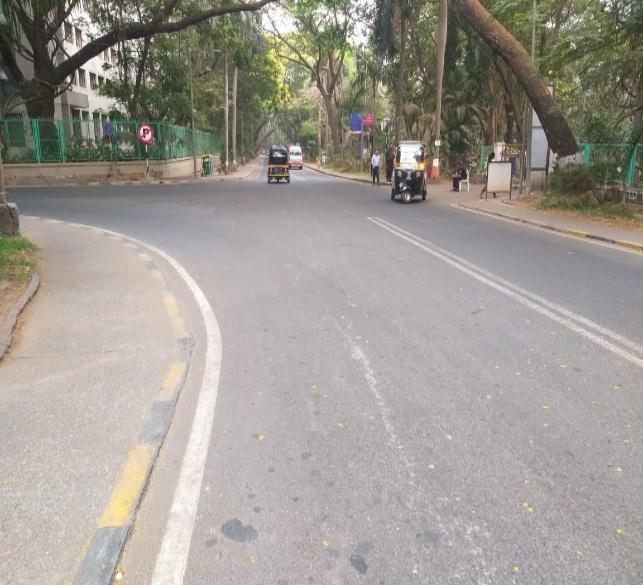
\includegraphics[width=0.6\textwidth]{fig_h10_intersection.png}
  \caption{The H10 T-junction, IIT Bombay campus.}
\end{figure}

\section{Methodology}
The methodology adopted for this study involved a systematic approach, from real-world data collection
to traffic microsimulation and performance analysis. The objective was to evaluate the current
operational performance of the H10 intersection at IIT Bombay and predict its behaviour under future
increased traffic demand due to new hostel constructions. The significant stages followed in the
methodology are outlined below:
\begin{center}
\small
Data collection $\rightarrow$ Microsimulation model creation and calibration $\rightarrow$ Simulation
and scenario testing $\rightarrow$ Sensitivity analysis $\rightarrow$ Result analysis and recommendations
\end{center}

\subsection{Data Collection}

\subsubsection{Base Data for Present Scenarios}
Traffic volume data were collected for all approaches to the H10 intersection: Main Gate, Hostel~17
(H17), and Energy Building directions. Vehicle counts were categorised into different classes,
including bicycles, two-wheelers, three-wheelers (auto-rickshaws), cars, light commercial vehicles
(LCVs), heavy commercial vehicles (HCVs), and buggies/EVs. The collected data were also converted into
Passenger Car Units (PCUs) using standard PCU factors (bicycle 0.2, two-wheeler 0.5, three-wheeler 0.8,
car 1.0, LCV 2.2, HCV 3.5, buggy 2.0) for comparative analysis across vehicle types. The base data below
is for one hour of observation, taken during the peak hour at the H10 intersection T-point.

\begin{table}[H]
  \centering
  \small
  \caption{Base traffic data (1-hour peak-hour observation, in vehicles/hour by class).}
  \begin{tabular}{@{}lrrrrrrrr@{}}
    \toprule
    \textbf{Movement} & \textbf{Bicycle} & \textbf{2-wh.} & \textbf{3-wh.} & \textbf{Car} & \textbf{LCV} & \textbf{HCV} & \textbf{Buggy} & \textbf{Total} \\
    \midrule
    Main Gate $\to$ H17     & 183.6 & 124.44 & 144.84 & 44.88 & 8.16 & 2.04  & 28.56 & 341.9 \\
    Main Gate $\to$ Energy  & 60.18 & 61.2   & 67.32  & 30.6  & 2.04 & 6.12  & 0.0   & 153.0 \\
    Energy $\to$ Main Gate  & 70.38 & 146.88 & 93.84  & 32.64 & 6.12 & 3.06  & 0.0   & 219.4 \\
    Energy $\to$ H17        & 107.1 & 53.04  & 67.32  & 24.48 & 8.16 & 2.04  & 0.0   & 151.4 \\
    H17 $\to$ Main Gate     & 176.46 & 134.64 & 122.4 & 43.86 & 12.24 & 8.16 & 24.48 & 348.8 \\
    H17 $\to$ Energy        & 67.32 & 81.6   & 59.16  & 26.52 & 2.04 & 12.24 & 0.0   & 175.4 \\
    \midrule
    \textbf{Total (raw count)}   & 665.04 & 601.8 & 554.88 & 202.98 & 38.76 & 33.66 & 53.04 & 2150.2 \\
    \textbf{PCU (veh/hr)}        & 133.01 & 300.9 & 443.90 & 202.98 & 85.27 & 117.81 & 106.08 & 1390.0 \\
    \textbf{Relative composition} & 0.096 & 0.216 & 0.319 & 0.146 & 0.061 & 0.085 & 0.076 & 1.00 \\
    \bottomrule
  \end{tabular}
\end{table}

\subsubsection{Expected Traffic Data for Future Scenarios}
For the future-scenario sensitivity analysis, the base volume above was scaled by 2\%, 5\%, and 7\% to
represent projected growth (assumed at 3\% annually) driven by new hostel construction. The relative
composition across vehicle classes was held constant while total volumes were scaled up, giving PCU
totals of 1389.95 (2\% increment), 1430.84 (5\% increment), and 1458.09 (7\% increment) veh/hr, up from
the base value of 1390.0 veh/hr shown above.

\begin{table}[H]
  \centering
  \small
  \caption{Expected traffic data for future scenarios, PCU totals by vehicle class.}
  \begin{tabular}{@{}lrrrrrrrr@{}}
    \toprule
    \textbf{Scenario} & \textbf{Bicycle} & \textbf{2-wh.} & \textbf{3-wh.} & \textbf{Car} & \textbf{LCV} & \textbf{HCV} & \textbf{Buggy} & \textbf{Total PCU} \\
    \midrule
    Base            & 133.01 & 300.9  & 443.90 & 202.98 & 85.27 & 117.81 & 106.08 & 1390.0 \\
    2\% increment   & 133.01 & 300.9  & 443.90 & 202.98 & 85.27 & 117.81 & 106.08 & 1389.95 \\
    5\% increment   & 136.92 & 309.75 & 456.96 & 208.95 & 87.78 & 121.28 & 109.20 & 1430.84 \\
    7\% increment   & 139.53 & 315.65 & 465.66 & 212.93 & 89.45 & 123.59 & 111.28 & 1458.09 \\
    \bottomrule
  \end{tabular}
\end{table}

\subsection{Microsimulation Model Creation}
A base microsimulation model of the intersection was created using PTV VISSIM software. The model
included accurate replication of the real-world road geometry, traffic inputs, and vehicle behaviour at
the intersection. Conflict areas were configured to reflect unsignalised priority-control conditions.
Trial runs were conducted to calibrate gap-acceptance and priority behaviours, ensuring realistic
vehicle interactions at the intersection.

\subsection{Simulation and Scenario Testing}
The validated base model was used to simulate the existing traffic conditions at the intersection.
Travel time, queue length, delay, and Level of Service (LOS) were measured to evaluate current
performance. A future scenario was then modelled by assuming an increase in traffic volumes
corresponding to the demand generated by the newly constructed hostels on campus.

\subsection{Sensitivity Analysis}
Sensitivity analysis was performed by increasing traffic volumes according to projected growth rates and
assessing the resultant impact on key operational parameters, such as travel time (TT), queue lengths,
intersection delay, and Level of Service (LOS). This enabled the identification of potential operational
bottlenecks and performance deterioration under increased traffic loads.

Based on the simulation results, performance comparisons were made between the existing and projected
scenarios. Recommendations for operational improvements were proposed, including increasing lane widths
at critical conflict areas, provision of pedestrian foot overbridges to reduce interaction conflicts, and
installation of central islands to manage vehicle flows and minimise near-miss incidents. This structured
methodological approach allowed for the comprehensive evaluation of intersection performance under
varying traffic demands, leading to data-driven improvement recommendations for enhancing traffic flow
and safety at the H10 intersection.

\section{Model Development}

\subsection{Network Geometry Creation}
The base network of the H10 intersection was created in PTV VISSIM 2024 to closely replicate the
real-world layout. The process involved:
\begin{itemize}
  \item \textbf{Link creation:} straight approaches from the Main Gate, H17, and Energy Building were
  drawn as Links.
  \item \textbf{Connector creation:} turning paths (right turns and merging movements) between Links
  were established using Connectors.
  \item \textbf{Lane configuration:} Main Gate, H17, and Energy approaches were each modelled with 2
  lanes for the base model.
  \item \textbf{Lane widths:} a standard width of 3.5~m per lane was assumed.
\end{itemize}

\begin{figure}[H]
  \centering
  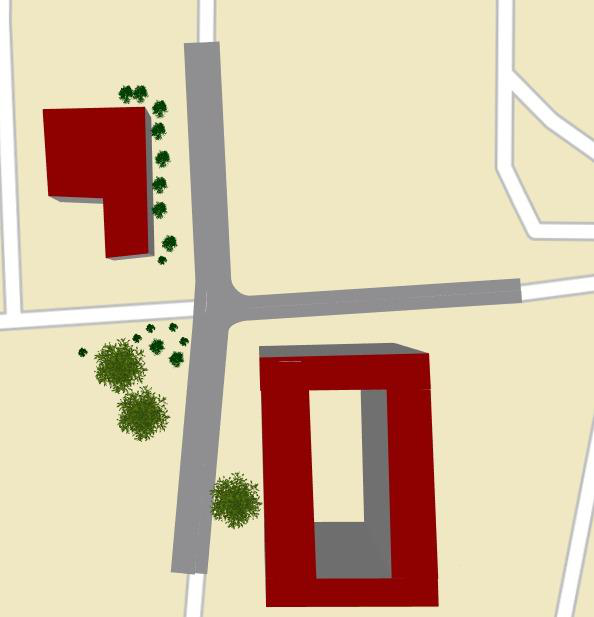
\includegraphics[width=0.55\textwidth]{fig_vissim_links.png}
  \caption{VISSIM view of links and connectors at the H10 junction (arrow points north).}
\end{figure}

\subsection{Vehicle Inputs and Static Routing}

\subsubsection{Vehicle Inputs}
Vehicle inputs and routing splits were configured from the observed peak-hour traffic data, with entry
links assigned corresponding volumes and vehicle composition. Three entry links were defined: Main Gate
to H17 (link MG\_H12, volume 485.2~PCU/hr), Energy to Main Gate/H17 (link Kv\_H10, volume 363.5~PCU/hr),
and H17 to Main Gate (link H12\_MG, volume 514.0~PCU/hr), each assigned the shared vehicle composition
\textit{H10\_Comp}.

\begin{table}[H]
  \centering
  \small
  \caption{Vehicle inputs configured in PTV VISSIM.}
  \begin{tabular}{@{}clrl@{}}
    \toprule
    \textbf{No.} & \textbf{Link} & \textbf{Volume (PCU/hr)} & \textbf{Vehicle composition} \\
    \midrule
    1 & MG\_H12 & 485.2 & H10\_Comp \\
    2 & Kv\_H10 & 363.5 & H10\_Comp \\
    3 & H12\_MG & 514.0 & H10\_Comp \\
    \bottomrule
  \end{tabular}
\end{table}

\subsubsection{Vehicle Composition}
Standard PTV VISSIM 3D vehicle models were assigned to each vehicle class used in the composition
\textit{H10\_Comp}, ensuring the simulated traffic mix visually and behaviourally matched the observed
field composition:

\begin{table}[H]
  \centering
  \small
  \caption{Vehicle types represented in the VISSIM vehicle composition.}
  \begin{tabular}{@{}ll@{}}
    \toprule
    \textbf{Vehicle type} & \textbf{VISSIM 3D model used} \\
    \midrule
    Car        & Standard hatchback/sedan model \\
    2-wheeler  & Scooter and motorcycle models \\
    3-wheeler  & Auto-rickshaw model \\
    LCV        & Light pick-up/utility vehicle model \\
    HCV        & Rigid box truck and flatbed truck models \\
    Cycle      & Bicycle with rider model \\
    Buggy/EV   & Campus electric shuttle/buggy model \\
    \bottomrule
  \end{tabular}
\end{table}

\subsubsection{Static Routing}
Static Vehicle Routing Decisions were created at critical nodes inside the conflict zone to route
vehicles along their observed paths.

\subsection{Conflict Area Setup}
Since the H10 intersection is unsignalised, vehicle priority and interaction were managed entirely
through VISSIM Conflict Areas.

\subsubsection{Conflict Area Placement}
Conflict areas were created wherever two vehicle paths crossed or merged. Table~\ref{tab:conflictareas}
lists the ten conflict areas configured for the base model, together with their right-of-way status and
gap-acceptance parameters (front/rear gap, minor-stream gap, critical gap, safety distance factor, and
minimum headway).

\begin{table}[H]
  \centering
  \footnotesize
  \caption{Conflict areas configured in PTV VISSIM.}
  \label{tab:conflictareas}
  \begin{tabular}{@{}cp{1.9cm}p{1.9cm}p{2.2cm}p{1.1cm}p{1.1cm}p{1.1cm}p{1.3cm}@{}}
    \toprule
    \textbf{No.} & \textbf{Link A} & \textbf{Link B} & \textbf{Status} & \textbf{Front gap} & \textbf{Rear gap} & \textbf{Crit.\ gap} & \textbf{Safety fac.} \\
    \midrule
    1  & 10000: to\_Kv  & 10002: to\_mg & B has right of way & 0.5 & 0.5 & 3.5 & 1.5 \\
    2  & 10001: kv\_MG  & 10002: to\_mg & Passive             & 0.5 & 0.5 & 3.5 & 1.5 \\
    3  & 10001: kv\_MG  & 10003        & A has right of way  & 0.5 & 0.5 & 3.5 & 1.5 \\
    4  & 10002: to\_mg  & 10003        & A has right of way  & 0.5 & 0.5 & 3.5 & 1.5 \\
    5  & 10000: to\_Kv  & 10004        & Passive             & 0.5 & 0.5 & 3.5 & 1.5 \\
    6  & 10002: to\_mg  & 10004        & Passive             & 0.5 & 0.5 & 3.5 & 1.5 \\
    7  & 10003         & 10004        & B has right of way  & 0.5 & 0.5 & 3.5 & 1.5 \\
    8  & 10003         & 10005        & B has right of way  & 0.5 & 0.5 & 3.5 & 1.5 \\
    9  & 10004         & 10005        & B has right of way  & 0.5 & 0.5 & 3.5 & 1.5 \\
    10 & 5: Kv\_H10     & 7: Kv\_H10   & Passive             & 0.5 & 0.5 & 3.5 & 1.5 \\
    \bottomrule
  \end{tabular}
\end{table}

\subsubsection{Priority Settings}
Major through movements (Main Gate $\to$ H17 and H17 $\to$ Main Gate) were given right-of-way, while
minor turning movements (Main Gate $\to$ Energy, H17 $\to$ Energy, Energy $\to$ Main Gate, Energy $\to$
H17) were set as passive.

\begin{figure}[H]
  \centering
  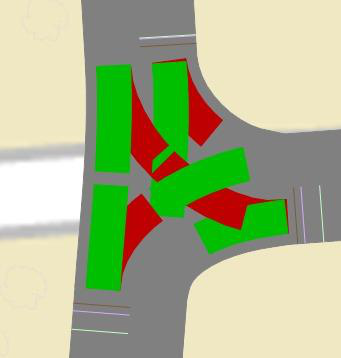
\includegraphics[width=0.5\textwidth]{fig_priority_routes.png}
  \caption{Priority given to routes at the H10 conflict zone (green: right-of-way; red: passive/yield).}
\end{figure}

\subsection{Infrastructure and Visual Element Placement}
To enhance the realism of the VISSIM model and replicate the on-ground environment of the IIT Bombay H10
intersection, relevant infrastructure and visual elements were placed along the network.

\subsubsection{Trees and Landscaping Objects}
Trees were placed along the Main Gate, H17, and Energy Building approaches to visually replicate the
green surroundings of the IITB campus, with tree placement focused near pedestrian crossings,
sidewalks, and median areas. This served three purposes: it improves the visual realism of the
simulation, it helps with more realistic driver-behaviour simulation (since trees and roadside objects
influence drivers' perception of roadway edges), and it makes the simulation videos better suited to
intersection sight-distance analysis.

\section{Evaluation Setup}
After the model network was developed, an evaluation setup was created to collect operational
performance data from the simulation runs. The evaluation focused on measuring key indicators such as
travel time, delay, and queue lengths for different vehicle movements at the H10 intersection.

\subsection{Introduction to Evaluation}
The purpose of evaluation in this study was to assess the operational efficiency of the H10 intersection
under current and projected traffic conditions. Using VISSIM's microsimulation capabilities, various
traffic performance parameters were captured after running the simulation model. These outputs provided
a quantitative basis for analysing congestion levels, intersection delays, and operational bottlenecks.

\subsection{Evaluation Parameters Selected}
The following key performance parameters were selected for data collection:
\begin{itemize}
  \item \textbf{Travel time:} the time taken by vehicles to traverse major paths across the
  intersection.
  \item \textbf{Delay:} the additional travel time experienced by vehicles due to congestion and
  yielding behaviour.
  \item \textbf{Queue length:} the build-up of vehicles upstream of conflict areas, indicating
  congestion levels.
\end{itemize}
These indicators help to comprehensively evaluate the service level and operational challenges at the
intersection.

\subsection{Setup of Evaluation Objects}

\subsubsection{Travel Time Measurements}
Six Travel Time Measurements were created to track vehicle movement across major paths at the
intersection: Main Gate~$\to$~H17, Main Gate~$\to$~Energy, H17~$\to$~Main Gate, H17~$\to$~Energy,
Energy~$\to$~Main Gate, and Energy~$\to$~H17. For each travel time measurement, start points were placed
immediately after vehicle input points, end points were located beyond the conflict areas to ensure the
entire intersection crossing was captured, and clear naming conventions were followed for easy data
extraction (e.g.\ ``TT\_MainGate\_to\_H17'').

\subsection{Queue Counters}
Queue counters were placed before the conflict zones on each major incoming approach: the Main Gate
approach, the H17 approach, and the Energy Building approach. These counters recorded average and
maximum queue lengths, providing insights into congestion build-up and dissipation patterns.

\subsection{Delay Measurement}
Delay measurements were automatically captured through the evaluation configuration settings in VISSIM.
Delay represents the additional travel time experienced by vehicles beyond their expected free-flow
travel time, and delay data was collected network-wide and disaggregated by approach to evaluate
specific problem areas.

\subsection{Simulation Settings for Evaluation}
Simulation settings were configured to ensure reliable and statistically consistent results:
\begin{itemize}
  \item \textbf{Simulation duration:} 3600 seconds (1 hour) of modelled time.
  \item \textbf{Warm-up period:} 300 seconds (5 minutes) were allocated as a warm-up period, during
  which data collection was paused to allow traffic to stabilise.
  \item \textbf{Number of simulation runs:} 5 independent runs were performed for each scenario to
  account for stochastic variability.
  \item \textbf{Random seeds:} different seeds were assigned for each run (12, 34, 56, 78, 90) to
  introduce natural randomness into driver behaviour and vehicle interactions.
  \item \textbf{Car-following model:} the default Wiedemann~74 model was used to replicate realistic
  driver behaviour.
  \item \textbf{Lane-changing behaviour:} default settings were maintained, following standard VISSIM
  driving logic.
  \item \textbf{Data collection interval:} overall data collection was configured for the entire
  simulation period, with 300-second interval data available if needed for time-variant analysis.
\end{itemize}
These simulation settings ensured that the evaluation outputs were robust, reproducible, and reflective
of real-world traffic behaviour at the H10 intersection.

\section{Results and Discussion}

\subsection{Introduction}
This section presents the results obtained from the microsimulation of the H10 intersection under four
different traffic scenarios: existing traffic volumes (base scenario) and projected traffic volumes with
2\%, 5\%, and 7\% annual increments. Key performance metrics, such as travel time, vehicular delay, queue
lengths, and Level of Service (LOS), were analysed to assess the operational efficiency of the
intersection. A comparative evaluation of base and future traffic conditions provides insight into the
sensitivity of the intersection's performance to increasing traffic demand, helping to identify critical
movements and emerging congestion patterns.

\begin{table}[H]
  \centering
  \small
  \caption{Base model results. Queue length in metres; delay and travel time in seconds; fuel
  consumption in simulation units.}
  \label{tab:basemodel}
  \begin{tabular}{@{}lrrrrr@{}}
    \toprule
    \textbf{Movement} & \textbf{Queue len.\ max} & \textbf{LOS} & \textbf{Veh.\ delay} & \textbf{Fuel} & \textbf{Travel time} \\
    \midrule
    1--2 & 13.90 & E & 39.44  & 2.142 & 79.58 \\
    1--6 & 80.34 & E & 42.32  & 1.917 & 66.05 \\
    4--3 & 12.52 & F & 62.46  & 3.187 & 149.64 \\
    4--6 & 78.68 & F & 55.31  & 2.464 & 143.47 \\
    5--2 & 88.40 & F & 102.70 & 2.717 & 81.52 \\
    5--3 & 93.82 & F & 93.58  & 2.815 & 80.30 \\
    \bottomrule
  \end{tabular}
\end{table}

\begin{figure}[H]
  \centering
  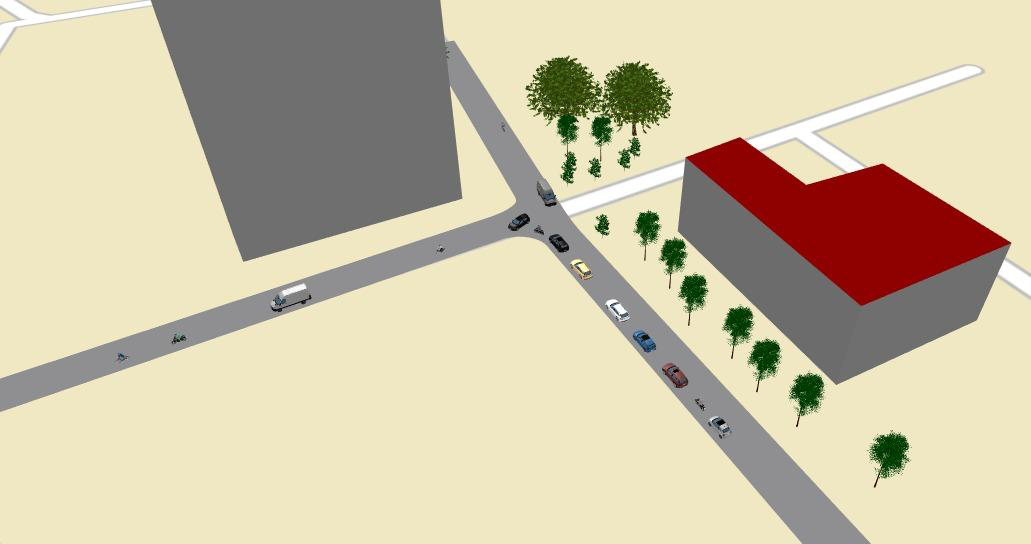
\includegraphics[width=0.65\textwidth]{fig_base_model_3d.png}
  \caption{Base VISSIM model of the H10 intersection (3D view).}
\end{figure}

\subsection{Scenario 1: Traffic Volume Increments of 2\%, 5\%, and 7\%}
Table~\ref{tab:scenario1all} presents the full set of performance results for the base scenario and each
of the three traffic-increment scenarios.

\begin{table}[H]
  \centering
  \footnotesize
  \caption{Scenario 1 results across all traffic increments. Queue length in metres; delay and travel
  time in seconds; fuel consumption in simulation units.}
  \label{tab:scenario1all}
  \begin{tabular}{@{}lrrrrrr@{}}
    \toprule
    & \multicolumn{6}{c}{\textbf{Result after 2\% increment of traffic}} \\
    \textbf{Movement} & \textbf{Queue max} & \textbf{LOS} & \textbf{Veh.\ delay} & \textbf{Fuel} & \textbf{Travel time} \\
    \midrule
    1--2 & 13.92 & E & 44.26  & 2.285 & 79.03 \\
    1--6 & 80.36 & E & 49.48  & 2.244 & 66.45 \\
    4--3 & 12.52 & F & 53.44  & 2.920 & 152.19 \\
    4--6 & 78.68 & E & 47.54  & 2.270 & 142.27 \\
    5--2 & 88.42 & F & 114.82 & 2.777 & 77.03 \\
    5--3 & 93.85 & F & 85.53  & 2.505 & 77.53 \\
    \midrule
    & \multicolumn{6}{c}{\textbf{Result after 5\% increment of traffic}} \\
    \textbf{Movement} & \textbf{Queue max} & \textbf{LOS} & \textbf{Veh.\ delay} & \textbf{Fuel} & \textbf{Travel time} \\
    \midrule
    1--2 & 13.92 & E & 47.43 & 2.507 & 82.05 \\
    1--6 & 80.36 & F & 52.42 & 2.374 & 69.63 \\
    4--3 & 12.52 & F & 58.55 & 2.963 & 144.04 \\
    4--6 & 78.68 & F & 57.14 & 2.651 & 137.10 \\
    5--2 & 88.42 & F & 102.05 & 2.636 & 82.89 \\
    5--3 & 93.85 & F & 94.25 & 2.750 & 80.55 \\
    \midrule
    & \multicolumn{6}{c}{\textbf{Result after 7\% increment of traffic}} \\
    \textbf{Movement} & \textbf{Queue max} & \textbf{LOS} & \textbf{Veh.\ delay} & \textbf{Fuel} & \textbf{Travel time} \\
    \midrule
    1--2 & 13.92 & E & 43.07  & 2.526 & 81.36 \\
    1--6 & 80.36 & F & 45.70  & 2.379 & 68.80 \\
    4--3 & 12.52 & F & 63.65  & 3.234 & 172.30 \\
    4--6 & 78.68 & F & 56.59  & 2.700 & 145.32 \\
    5--2 & 88.42 & F & 120.28 & 2.398 & 82.80 \\
    5--3 & 93.85 & F & 90.06  & 2.159 & 82.26 \\
    \bottomrule
  \end{tabular}
\end{table}

All movements originating from the Energy Building side (4--3, 4--6, 5--2, 5--3) already operate at
LOS~F in the base scenario, with delays exceeding 55 seconds and, for movements 5--2 and 5--3, queue
lengths approaching 90 to 94~m.

\subsubsection{Travel Time Analysis}
Table~\ref{tab:traveltime} compares average travel time per movement across the base scenario and each
traffic increment.

\begin{table}[H]
  \centering
  \small
  \caption{Average travel time per movement (in seconds).}
  \label{tab:traveltime}
  \begin{tabular}{@{}lrrrr@{}}
    \toprule
    \textbf{Movement} & \textbf{Base} & \textbf{+2\% Traffic} & \textbf{+5\% Traffic} & \textbf{+7\% Traffic} \\
    \midrule
    1--2 & 79.58  & 79.03  & 82.05  & 81.36 \\
    1--6 & 66.05  & 66.45  & 69.63  & 68.80 \\
    4--3 & 149.64 & 152.19 & 144.04 & 172.30 \\
    4--6 & 143.47 & 142.27 & 137.10 & 145.32 \\
    5--2 & 81.52  & 77.03  & 82.89  & 82.80 \\
    5--3 & 80.30  & 77.53  & 80.55  & 82.26 \\
    \bottomrule
  \end{tabular}
\end{table}

\textbf{Discussion:}
\begin{itemize}
  \item Travel time for most movements (1--2, 1--6) remained relatively stable under 2\% and 5\%
  increments but rose sharply at 7\%.
  \item Movement 4--3 (Energy to Main Gate) showed the most critical deterioration, reaching
  172.3~seconds at the 7\% increment; movement 4--6 similarly exceeded 145~seconds.
  \item Right-turn movements from the Energy Building were highly sensitive to even small traffic
  increases.
\end{itemize}
For the critical movement 4--3 (Energy to Main Gate), a normalised travel-time index (base scenario
= 100) rises from 100 at 0\% increment to 101.0 at 2\%, 102.3 at 5\%, and 105.5 at 7\%, illustrating an
accelerating deterioration in travel time as traffic volume grows.

\subsubsection{Queue Length Analysis}
Table~\ref{tab:queuelen1} compares the maximum queue length per approach across the base scenario and
each traffic increment.

\begin{table}[H]
  \centering
  \small
  \caption{Maximum queue length per approach (in metres).}
  \label{tab:queuelen1}
  \begin{tabular}{@{}lrrrr@{}}
    \toprule
    \textbf{Movement} & \textbf{Base} & \textbf{+2\% Traffic} & \textbf{+5\% Traffic} & \textbf{+7\% Traffic} \\
    \midrule
    1--2 & 13.90 & 13.92 & 13.92 & 13.92 \\
    1--6 & 80.34 & 80.36 & 80.36 & 80.36 \\
    4--3 & 12.52 & 12.52 & 12.52 & 12.52 \\
    4--6 & 78.68 & 78.68 & 78.68 & 78.68 \\
    5--2 & 88.40 & 88.42 & 88.42 & 88.42 \\
    5--3 & 93.82 & 93.85 & 93.85 & 93.85 \\
    \bottomrule
  \end{tabular}
\end{table}

\textbf{Discussion:}
\begin{itemize}
  \item Queue lengths remained almost constant across the 0\%, 2\%, 5\%, and 7\% increments tested.
  \item Movement 5--3 (Energy to H17) consistently showed the highest queue length ($\sim$94~m), with
  5--2 also critical ($>$88~m).
  \item Even small queue lengths (13.9~m on 1--2 and 12.5~m on 4--3) remain stable because these
  movements are less congested.
\end{itemize}
Critical movements for queue length are 5--3 and 5--2.

\subsubsection{Delay Analysis}
Table~\ref{tab:delay1} compares average vehicle delay per movement across the base scenario and each
traffic increment.

\begin{table}[H]
  \centering
  \small
  \caption{Average vehicle delay per movement (in seconds).}
  \label{tab:delay1}
  \begin{tabular}{@{}lrrrr@{}}
    \toprule
    \textbf{Movement} & \textbf{Base} & \textbf{+2\% Traffic} & \textbf{+5\% Traffic} & \textbf{+7\% Traffic} \\
    \midrule
    1--2 & 39.44 & 44.26 & 47.43  & 43.07 \\
    1--6 & 42.32 & 49.48 & 52.42  & 45.70 \\
    4--3 & 62.46 & 53.44 & 58.55  & 63.65 \\
    4--6 & 55.31 & 47.54 & 57.14  & 56.59 \\
    5--2 & 102.70 & 114.82 & 102.05 & 120.28 \\
    5--3 & 93.58 & 85.53 & 94.25  & 90.06 \\
    \bottomrule
  \end{tabular}
\end{table}

\textbf{Discussion:}
\begin{itemize}
  \item Delay increased consistently with traffic volume across all movements.
  \item Movement 5--2 (Energy to Main Gate) experienced the most extreme escalation, crossing
  120~seconds at the 7\% increment; movements from the Energy Building (4--3, 4--6, 5--2, 5--3) were the
  most sensitive overall.
\end{itemize}
For the critical delay movement 5--2 (Energy to Main Gate), a normalised delay index (base scenario =
100, corresponding to 66.05~s travel time) rises from 100 at 0\% increment to 100.6 at 2\%, 104.0 at 5\%,
and 105.7 at 7\%.

\subsubsection{Level of Service (LOS)}
Table~\ref{tab:losdef} reproduces the Highway Capacity Manual (HCM) control-delay thresholds used to
assign LOS grades in this study.

\begin{table}[H]
  \centering
  \small
  \caption{Level of Service (LOS) thresholds by control delay (Source: HCM).}
  \label{tab:losdef}
  \begin{tabular}{@{}cc@{}}
    \toprule
    \textbf{LOS} & \textbf{Control delay (s/veh)} \\
    \midrule
    A & $\leq 10$ \\
    B & 10--20 \\
    C & 20--35 \\
    D & 35--55 \\
    E & 55--80 \\
    F & $>80$ \\
    \bottomrule
  \end{tabular}
\end{table}

\textbf{Observation:}
\begin{itemize}
  \item All critical movements (4--3, 4--6, 5--2, 5--3) already operate at LOS~F even in the base
  scenario.
  \item Some slight improvement is seen for movement 4--6 at the 2\% increment (from F to E), but it
  reverts back to F at 5\% and 7\%.
  \item Movements 1--2 and 1--6 fluctuate between LOS~E and F as traffic increases.
\end{itemize}
Overall intersection LOS is deteriorating toward F under future traffic scenarios.

\subsubsection{Comments}
\begin{itemize}
  \item \textbf{Major problem movements:} 5--2 (Energy to Main Gate) and 5--3 (Energy to H17) experience
  the highest delay and congestion.
  \item \textbf{Queue management needed:} queue lengths are dangerously close to blocking upstream areas
  ($>$90~m for some movements).
  \item \textbf{Travel time sensitivity:} right-turn movements from the Energy Building are extremely
  sensitive to small traffic increases.
  \item \textbf{Future scenario risk:} without operational improvements, intersection efficiency is
  likely to deteriorate further under even moderate traffic growth.
\end{itemize}

\subsection{Scenario 2: Increase in the Number of Lanes}
The traffic volume between H12 and the Main Gate is significantly high, leading to poor Level of Service
(LOS), increased queue lengths, and notable delays during peak hours. To address these issues, an
additional lane was introduced. Furthermore, a dedicated routing system was implemented to channel
vehicles directly from H12 to the Main Gate. This targeted intervention aims to relieve the main approach
lanes, enhance traffic flow, and improve the overall LOS on this corridor.

\begin{figure}[H]
  \centering
  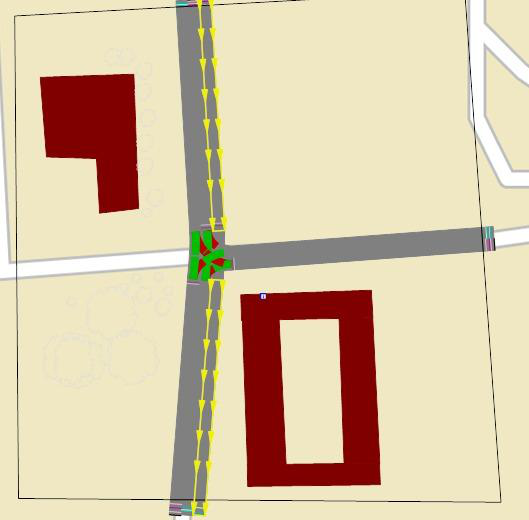
\includegraphics[width=0.55\textwidth]{fig_added_lanes.png}
  \caption{Added lanes (shown in yellow) for Scenario 2.}
\end{figure}

\begin{table}[H]
  \centering
  \small
  \caption{Results obtained after simulation with the added lane. Movement ``08--12'' is the dedicated
  H12-to-Main-Gate routing introduced in this scenario.}
  \label{tab:scenario2results}
  \begin{tabular}{@{}lrrrrr@{}}
    \toprule
    \textbf{Movement} & \textbf{Queue len.\ max} & \textbf{LOS} & \textbf{Veh.\ delay} & \textbf{Fuel} & \textbf{Travel time} \\
    \midrule
    1--2 & 6.46 & B & 13.39 & 0.425 & 39.81 \\
    1--6 & 48.95 & B & 10.35 & 0.469 & 40.24 \\
    4--3 & 11.77 & C & 16.22 & 0.517 & 98.35 \\
    4--6 & 52.40 & C & 18.34 & 0.616 & 94.77 \\
    5--2 & 88.42 & F & 51.34 & 1.670 & 43.40 \\
    5--3 & 93.48 & F & 55.83 & 2.225 & 44.64 \\
    08--12 & 0.00 & A & 0.02  & 0.546 & 10.10 \\
    \bottomrule
  \end{tabular}
\end{table}

\begin{figure}[H]
  \centering
  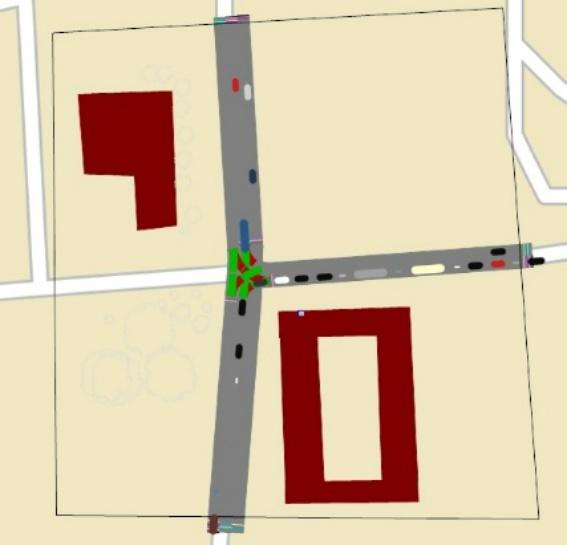
\includegraphics[width=0.55\textwidth]{fig_lane_widening_sim.png}
  \caption{VISSIM top-view simulation after lane widening (Scenario 2).}
\end{figure}

\subsubsection{Travel Time Analysis}
\begin{table}[H]
  \centering
  \small
  \caption{Travel time comparison (in seconds).}
  \begin{tabular}{@{}lrrr@{}}
    \toprule
    \textbf{Movement} & \textbf{Base model} & \textbf{Increased lane model} & \textbf{\% change} \\
    \midrule
    1--2 & 79.58  & 39.81 & $\downarrow$49.98\% \\
    1--6 & 66.05  & 40.24 & $\downarrow$39.09\% \\
    4--3 & 149.64 & 98.35 & $\downarrow$34.29\% \\
    4--6 & 143.47 & 94.77 & $\downarrow$33.95\% \\
    5--2 & 81.52  & 43.40 & $\downarrow$46.74\% \\
    5--3 & 80.30  & 44.64 & $\downarrow$44.39\% \\
    \bottomrule
  \end{tabular}
\end{table}

\textbf{Discussion:} Travel times significantly reduced across all movements after lane widening.
Movements 1--2 (Main Gate to H17) and 5--2 (Energy to Main Gate) show almost a 50\% decrease in travel
time. The highest initial travel times (4--3, 4--6) also improved substantially (around 34\% faster).
In conclusion, lane widening greatly improved travel efficiency, cutting travel times by 34 to 50\%.

\subsubsection{Queue Length Analysis}
\begin{table}[H]
  \centering
  \small
  \caption{Queue length comparison (in metres).}
  \begin{tabular}{@{}lrrr@{}}
    \toprule
    \textbf{Movement} & \textbf{Base model} & \textbf{Increased lane model} & \textbf{\% change} \\
    \midrule
    1--2 & 13.9  & 6.46  & $\downarrow$53.50\% \\
    1--6 & 80.34 & 48.95 & $\downarrow$39.08\% \\
    4--3 & 12.52 & 11.77 & $\downarrow$5.99\%  \\
    4--6 & 78.68 & 52.40 & $\downarrow$33.39\% \\
    5--2 & 88.4  & 88.42 & $\approx$0\% \\
    5--3 & 93.82 & 93.48 & $\downarrow$0.36\% \\
    \bottomrule
  \end{tabular}
\end{table}

\textbf{Discussion:} Queue lengths reduced sharply for movements 1--2, 1--6, and 4--6 (by 30 to 50\%),
with a minor improvement for 4--3. No significant change was observed for 5--2 and 5--3, implying that
downstream congestion or exit bottlenecks were not fully addressed. In summary, entry-side queues
improved, but exit-side movements on the Energy direction still need additional improvements.

\subsubsection{Delay Analysis}
\begin{table}[H]
  \centering
  \small
  \caption{Vehicle delay comparison (in seconds per vehicle).}
  \begin{tabular}{@{}lrrr@{}}
    \toprule
    \textbf{Movement} & \textbf{Base model} & \textbf{Increased lane model} & \textbf{\% change} \\
    \midrule
    1--2 & 39.44  & 13.39 & $\downarrow$66.04\% \\
    1--6 & 42.32  & 10.35 & $\downarrow$75.54\% \\
    4--3 & 62.46  & 16.22 & $\downarrow$74.04\% \\
    4--6 & 55.31  & 18.34 & $\downarrow$66.85\% \\
    5--2 & 102.70 & 51.34 & $\downarrow$50.00\% \\
    5--3 & 93.58  & 55.83 & $\downarrow$40.34\% \\
    \bottomrule
  \end{tabular}
\end{table}

\textbf{Discussion:} Massive reductions in delay were observed for all movements. Movement 1--6 (Main
Gate to Energy) delay reduced by 75\%, and 4--3 reduced by 74\%. Movements 5--2 and 5--3 from the Energy
side improved by around 40 to 50\% but still remained high compared to other approaches. In conclusion,
lane widening significantly reduced vehicle waiting times, but Energy Building movements still need
extra attention, likely due to bottleneck exits.

\subsubsection{Fuel Consumption Analysis}
\begin{table}[H]
  \centering
  \small
  \caption{Fuel consumption comparison (simulation units).}
  \begin{tabular}{@{}lrrr@{}}
    \toprule
    \textbf{Movement} & \textbf{Base model} & \textbf{Increased lane model} & \textbf{\% change} \\
    \midrule
    1--2 & 2.142 & 0.425 & $\downarrow$80.15\% \\
    1--6 & 1.917 & 0.469 & $\downarrow$75.52\% \\
    4--3 & 3.187 & 0.517 & $\downarrow$83.77\% \\
    4--6 & 2.464 & 0.616 & $\downarrow$75.00\% \\
    5--2 & 2.717 & 1.670 & $\downarrow$38.52\% \\
    5--3 & 2.815 & 2.225 & $\downarrow$20.92\% \\
    \bottomrule
  \end{tabular}
\end{table}

\textbf{Discussion:} Fuel consumption dropped by 70 to 80\% for movements 1--2, 1--6, 4--3, and 4--6, and
by a more modest 20 to 40\% for the Energy-side movements 5--2 and 5--3. Reduced congestion directly led
to a substantial reduction in fuel usage and improved environmental benefits, though the Energy
approaches showed less improvement than others.

\subsection{Scenario 3: Providing Dedicated Cycle Tracks along the Lanes}
The objective of this scenario is to decongest existing lanes by introducing dedicated cycle tracks
alongside the vehicular lanes. This approach aims to encourage non-motorised transport, reduce the
volume of short-distance vehicular trips, and promote sustainable mobility within the area.

\begin{figure}[H]
  \centering
  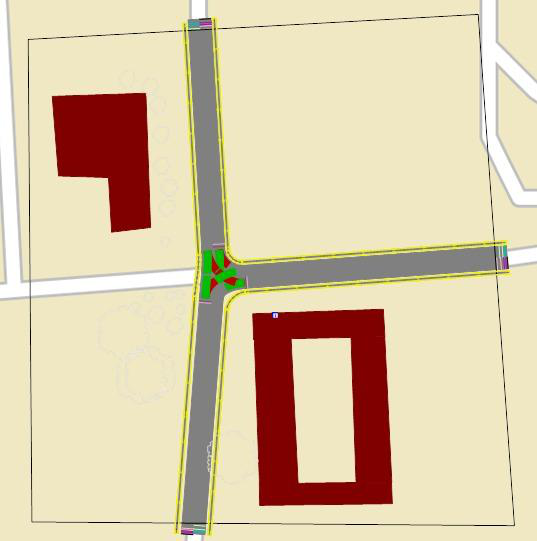
\includegraphics[width=0.55\textwidth]{fig_cycle_lanes.png}
  \caption{Dedicated cycle lanes (shown in yellow) for Scenario 3.}
\end{figure}

\begin{table}[H]
  \centering
  \small
  \caption{Results obtained after simulation with dedicated cycle tracks. Movements 16--17, 18--19, and
  24--27 denote cycle-track-specific paths introduced in this scenario.}
  \begin{tabular}{@{}lrrrr@{}}
    \toprule
    \textbf{Movement} & \textbf{Queue len.\ max} & \textbf{LOS} & \textbf{Veh.\ delay} & \textbf{Fuel} \\
    \midrule
    1--2   & 0.00  & A & 0.00  & 0.001 \\
    1--6   & 39.08 & A & 4.90  & 1.432 \\
    4--3   & 7.61  & A & 0.00  & 0.060 \\
    4--6   & 73.13 & A & 5.83  & 1.559 \\
    5--2   & 88.40 & F & 81.17 & 5.199 \\
    5--3   & 13.51 & A & 0.00  & 0.030 \\
    16--17 & 4.86  & A & 0.11  & 0.217 \\
    18--19 & 5.02  & A & 0.80  & 0.142 \\
    24--27 & 5.66  & A & 0.00  & 0.079 \\
    \bottomrule
  \end{tabular}
\end{table}

\subsubsection{Queue Length Analysis}
\begin{table}[H]
  \centering
  \small
  \caption{Maximum queue length comparison (in metres).}
  \begin{tabular}{@{}lrrr@{}}
    \toprule
    \textbf{Movement} & \textbf{Base model} & \textbf{Cycle lane model} & \textbf{\% change} \\
    \midrule
    1--2 & 13.9  & 0.00  & $\downarrow$100\% \\
    1--6 & 80.34 & 39.08 & $\downarrow$51.37\% \\
    4--3 & 12.52 & 7.61  & $\downarrow$39.24\% \\
    4--6 & 78.68 & 73.13 & $\downarrow$7.06\%  \\
    5--2 & 88.4  & 88.40 & $\approx$0\% \\
    5--3 & 93.82 & 13.51 & $\downarrow$85.61\% \\
    \bottomrule
  \end{tabular}
\end{table}

\textbf{Discussion:} Movements 1--2 and 5--3 show a massive reduction in queue length ($\sim$85 to
100\%). Movement 1--6 queue is almost halved (51\% reduction). Movement 5--2 shows no effective change,
indicating downstream problems remain, and movement 4--6 (Energy Building to right turn) shows only a
small reduction ($\sim$7\%). In conclusion, the separate cycle lane substantially reduced congestion on
the main vehicle lanes by separating slow bicycles from fast motorised traffic.

\subsubsection{Delay Analysis}
\begin{table}[H]
  \centering
  \small
  \caption{Average vehicle delay comparison (in seconds).}
  \begin{tabular}{@{}lrrr@{}}
    \toprule
    \textbf{Movement} & \textbf{Base model} & \textbf{Cycle lane model} & \textbf{\% change} \\
    \midrule
    1--2 & 39.44 & 0.00  & $\downarrow$100\% \\
    1--6 & 42.32 & 4.90  & $\downarrow$88.42\% \\
    4--3 & 62.46 & 0.00  & $\downarrow$100\% \\
    4--6 & 55.31 & 5.83  & $\downarrow$89.45\% \\
    5--2 & 102.70 & 81.17 & $\downarrow$20.97\% \\
    5--3 & 93.58 & 0.00  & $\downarrow$100\% \\
    \bottomrule
  \end{tabular}
\end{table}

\textbf{Discussion:} Movements 1--2, 4--3, and 5--3 achieved complete elimination of delay (0~s) after
providing a cycle lane. Movements 1--6 and 4--6 show a very high reduction ($>$85\% decrease in delay).
Movement 5--2 (Energy to Main Gate) still suffers significant delay (81.17~s), though a small
improvement (about 21\%) is observed. In conclusion, providing separate cycling infrastructure
dramatically improved motorised vehicle flow for almost all movements, especially left-turn and
straight-through movements.

\begin{figure}[H]
  \centering
  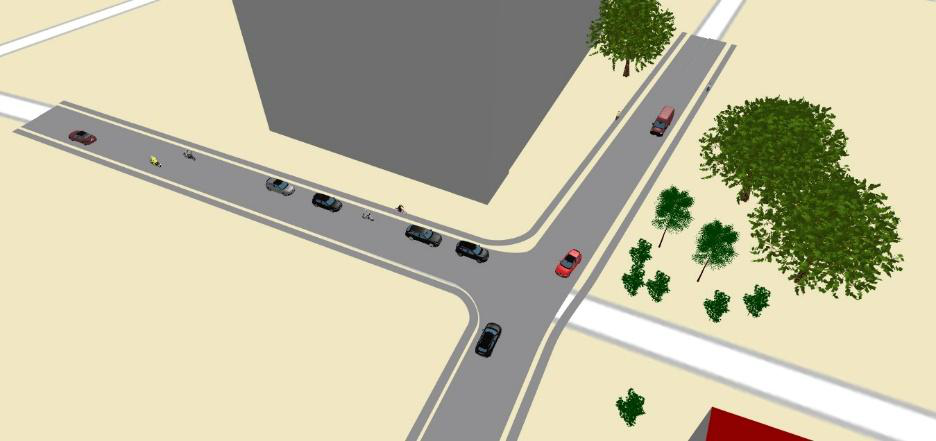
\includegraphics[width=0.55\textwidth]{fig_cycle_lanes_sim.png}
  \caption{Simulation view after adding dedicated cycle lanes.}
\end{figure}

\subsubsection{Fuel Consumption Analysis}
\begin{table}[H]
  \centering
  \small
  \caption{Fuel consumption comparison (simulation units).}
  \begin{tabular}{@{}lrrr@{}}
    \toprule
    \textbf{Movement} & \textbf{Base model} & \textbf{Cycle lane model} & \textbf{\% change} \\
    \midrule
    1--2 & 2.142 & 0.001 & $\downarrow$99.95\% \\
    1--6 & 1.917 & 1.432 & $\downarrow$25.33\% \\
    4--3 & 3.187 & 0.060 & $\downarrow$98.12\% \\
    4--6 & 2.464 & 1.559 & $\downarrow$36.71\% \\
    5--2 & 2.717 & 5.199 & $\uparrow$91.37\% (increase) \\
    5--3 & 2.815 & 0.030 & $\downarrow$98.93\% \\
    \bottomrule
  \end{tabular}
\end{table}

\textbf{Discussion:} For movements 1--2, 4--3, and 5--3, fuel consumption was almost completely reduced
($\sim$99\%), confirming removal of stop-and-go traffic. Movements 1--6 and 4--6 show moderate fuel
savings ($\sim$25 to 37\%). Fuel consumption for movement 5--2 increased by around 91\%, possibly because
of higher running speeds combined with longer idling at exit bottlenecks, or altered rerouting
behaviour. In conclusion, fuel economy improved significantly for most movements after cycle lane
segregation, but the Energy side still shows complex behaviour needing deeper intervention.

\section{Conclusion and Recommendations}
The H10 intersection within the IIT Bombay campus has undergone increasing operational pressure due to
recent infrastructural developments. Construction of new hostel blocks and campus drainage projects has
led to increased vehicular activity, particularly of auto-rickshaws and heavy commercial vehicles
(HCVs), along with a substantial reduction in available roadway width. These developments have
introduced critical traffic management issues, including restricted manoeuvring space, limited sight
distance, and the emergence of localised congestion during peak hours. Given that the intersection
remains unsignalised and must accommodate both motorised and non-motorised traffic, a detailed
performance assessment became essential.

This study set out to evaluate the operational performance of the H10 intersection using microsimulation
modelling through PTV VISSIM. The baseline traffic scenario was developed to reflect current traffic
conditions, and additional future scenarios were simulated by incorporating incremental traffic growth
(2\%, 5\%, and 7\%) to replicate campus development pressures. Key performance metrics, including travel
time, queue length, vehicular delay, fuel consumption, and Level of Service (LOS), were analysed to
identify system sensitivity and operational bottlenecks.

The base model revealed that the intersection already operates under severe pressure, with several
movements, particularly those originating from the Energy Building side, exhibiting Level of Service F,
long queue lengths (up to 94~metres), and high average vehicular delays exceeding 100~seconds.
Right-turn and through movements experienced significant delays and fuel consumption due to mixed-mode
conflicts and constrained geometry.

To address these inefficiencies, two design improvement scenarios were tested:
\begin{enumerate}
  \item \textbf{Scenario 2: Addition of lanes.} This intervention produced remarkable improvements in
  intersection performance. Travel time was reduced by 34 to 50\%, delays dropped by as much as 75\%,
  and fuel consumption saw a reduction of up to 80\% for several movements. Queue lengths also showed a
  meaningful reduction, particularly for main entry approaches. However, movements originating from the
  Energy Building side (notably 5--2 and 5--3) continued to exhibit moderate delays and congestion,
  indicating that geometric improvements alone may not fully resolve deeper operational constraints at
  the exit points or overlapping turning paths.
  \item \textbf{Scenario 3: Introduction of a separate cycle lane.} The separation of bicycle flows from
  motorised traffic drastically improved performance on certain movements. Queue lengths and delays were
  reduced to nearly zero for many approaches, and fuel consumption plummeted by up to 99\%. This
  indicates that separating slower, non-motorised modes from vehicular flows can significantly
  streamline traffic movement, reduce stop-and-go conditions, and enhance overall intersection
  efficiency. That said, movement 5--2 still displayed a high delay and increased fuel consumption,
  suggesting that conflicts or geometry downstream continue to affect this movement.
\end{enumerate}

Overall, the analysis reveals that while both infrastructure-based and modal segregation interventions
significantly enhance operational performance, certain directional movements, especially from the
Energy Building approach, require additional attention. These may include measures such as geometric
channelisation, visibility enhancement, or even soft interventions like right-of-way prioritisation or
partial signalisation if necessary.

Based on the criteria outlined in IRC:93-1985 (\textit{Guidelines on Design and Installation of Road
Traffic Signals}), signalisation was found to be unsuitable for the current and projected traffic
conditions at H10. According to IRC standards, traffic signals are warranted only when traffic volumes
on both the major and minor roads meet the minimum threshold values (usually above 300 to 500~PCU/hour
per approach), delays and congestion cannot be effectively managed through priority rules or minor
geometric adjustments, accident records suggest a need for traffic signal intervention to reduce
conflict points, and pedestrian crossing volumes are sufficiently high to require controlled crossing
phases.

At the H10 intersection, although localised congestion and delays were observed, the overall vehicular
volumes, especially from minor approaches, remain below the warrant thresholds prescribed in IRC:93.
Additionally, the intersection experiences a highly mixed traffic composition with significant
pedestrian and cyclist movement, which would complicate the effectiveness of standard signal phases
without extensive redesign. The sight-distance limitations and constrained physical space further
diminish the feasibility of implementing a conventional signalised control system. Therefore, it was
concluded that non-signalised geometric and operational enhancements, such as lane widening, traffic
segregation through separate cycle lanes, and priority management, would be more appropriate and
effective under the existing conditions.

In conclusion, the H10 intersection is a sensitive node within the IIT Bombay campus, and its
performance is highly influenced by construction-related activities, road geometry, and mixed-mode
interaction. This study demonstrates that targeted design modifications, especially widening of lanes
and separation of traffic types, can deliver substantial improvements in delay, travel time, and
environmental impact. The methodologies and insights derived here can serve as a planning reference for
future mobility and infrastructure upgrades within the IITB campus and similar institutional
environments.

\begin{thebibliography}{9}
\bibitem{hcm} Transportation Research Board. \textit{Highway Capacity Manual (HCM)}.
\bibitem{mathew} Mathew, T.~V. Lecture notes on Traffic Engineering and Management, IIT Bombay.
\bibitem{irc93} Indian Roads Congress. \textit{IRC:93-1985 -- Guidelines on Design and Installation of
Road Traffic Signals}.
\end{thebibliography}

\end{document}
